\documentclass{article}
\usepackage{graphicx}
\usepackage{amsmath}
\usepackage{mathtools}
\usepackage{pdfpages}
\usepackage{float}

\newcommand{\east}{e_e}
\newcommand{\north}{e_n}
\newcommand{\up}{e_u}
\newcommand{\range}{e_r}
\newcommand{\bearing}{e_\theta}
\newcommand{\elevation}{e_\phi}
\newcommand{\rrate}{\dot{r}}
\newcommand{\brate}{\dot{\theta}}
\newcommand{\erate}{\dot{\phi}}
\newcommand{\carvec}{\hat{e_{c}}}
\newcommand{\polvec}{\hat{e_{p}}}

\begin{document}

\section{Coordinate Conversions From Spherical to Cartesian}

\subsection{Notations}
\subsubsection{Spherical Coordinate system}
In the polar coordinate system we represent the location of the target in terms
of range, bearing and elevation. where range denotes the distance away from the
target's position, bearing denotes the angle to the target (taken from the north
axis), and elevation denotes the angle between the tanget plan and the target.


\subsubsection{Cooridnate system representation}

We denote by $\carvec=(\east,\north, \up)$ the column vector that represents
the the coordinate system in ENU terms. each $\east,\north, \up$ is a unit vector
which represents the distance in east direction, north direction and up
direction, respectively.

We denote by $\polvec=(\range,\bearing,\elevation)$ the column vector that
represents the the coordinate system in spherical terms. each $\range,\bearing,\elevation$ is a
unit vector which represents the distance in east direction, north direction and up
direction, respectively.

\subsection{Conversion from one system to the other}

\subsubsection{Position conversions}
Let $\vec{p} = (x,y,z) \cdot \carvec = x\east + y\north + z\up$ denote the
position of the target.


\paragraph{Conversion of position from spherical to cartesian:}
\begin{align}\label{eq:cartesian-position}
\begin{split}
{}& x=r\sin \theta \cos \phi \\
{}& y=r\cos \theta \cos \phi \\
{}& z=r\sin \phi
\end{split}
\end{align}


\paragraph{Conversion of position from cartesian to spherical:}
\begin{align}\label{eq:polar-position}
\begin{split}
{}& r= \sqrt{x^2 + y^2 + z^2} \\
{}& \theta= \arctan \frac{x}{y} \\
{}& \phi = \arctan \frac{z}{\sqrt{x^2 + y^2}}
\end{split}
\end{align}

\subsubsection{Unit conversions}
 We would like to convert the vector $\carvec$ to spherical
coordinates $\polvec$.

That is, $\vec{p} = r\sin \theta \cos \phi \east + r\cos \theta \cos \phi \north +
r\sin \phi \up = r( \sin \theta \cos \phi \east + \cos \theta \cos \phi \north +
\sin \phi \up)$

\begin{equation}
\vec{p} = r( \sin \theta \cos \phi \east + \cos \theta \cos \phi \north +
\sin \phi \up)
\end{equation}

And we obtain:
\begin{equation}\label{eq:range}
\range = \frac{\frac{\partial \vec{p}}{\partial r}}{\| \frac{\partial
\vec{p}}{\partial r} \|} = \sin \theta \cos \phi \east + \cos \theta \cos \phi \north +
\sin \phi \up 
\end{equation}

\begin{align}\label{eq:bearing}
\begin{split}
\bearing = \frac{\frac{\partial \vec{p}}{\partial \theta}}{\| \frac{\partial
\vec{p}}{\partial \theta} \|} = \frac{r( \cos \theta \cos \phi \east - \sin
\theta \cos \phi \north) }{r \| \cos \theta \cos \phi \east - \sin \theta
\cos \phi \north\|} = \\
= \frac{r( \cos \theta \cos \phi \east - \sin \theta
\cos \phi \north) }{r |\cos \phi |} = \cos \theta \east - \sin \theta \north
\end{split}
\end{align}

\begin{align}
\begin{split}
\elevation = \frac{\frac{\partial \vec{p}}{\partial \phi}}{\| \frac{\partial
\vec{p}}{\partial \phi} \|} = \frac{r( - \sin \theta \sin \phi \east - \cos
\theta \sin \phi \north + \cos \phi \up) }{r \| - \sin \theta \sin \phi \east - \cos
\theta \sin \phi \north + \cos \phi \up \|} = \\
= \frac{r( - \sin \theta \sin \phi \east - \cos
\theta \sin \phi \north + \cos \phi \up) }{r} = \\
= - \sin \theta \sin \phi \east
- \cos \theta \sin \phi \north + \cos \phi \up
\end{split}
\end{align}

Namely,

\begin{equation}\label{eq:matrix}
\begin{pmatrix}
    \range \\
   \bearing \\
    \elevation
  \end{pmatrix}
  \qquad
  = \begin{pmatrix}
    \sin \theta \cos \phi & \cos \theta \cos \phi &  \sin \phi \\
   \cos \theta &  -\sin \theta & 0 \\
    -\sin \theta \sin \phi & -\cos \theta \sin \phi &  \cos \phi
  \end{pmatrix}
  \qquad
  \begin{pmatrix}
    \east \\
   \north \\
    \up
  \end{pmatrix}
\end{equation}

In Equation~\ref{eq:bearing} we canceled the term $\cos \phi$
since it is always positive $\| \cos \phi \| = \cos \phi$.

Denote by $\Sigma$ the conversion matrix as described above, note that $\Sigma$
is unitary matrix.

\begin{equation}
\Sigma^{-1} = \begin{pmatrix}
    \sin \theta \cos \phi & \cos \theta &  - \sin \theta \sin \phi \\
   \cos \theta \cos \phi &  -\sin \theta & -\cos \theta \sin \phi \\
    \sin \phi & 0 &  \cos \phi
  \end{pmatrix}
\end{equation}

\subsubsection{Velocity conversions}
Let $\vec{v}$ denote the velocity vector. We denote by $\rrate, \brate, \erate$ the terms: range-rate, bearing-rate,
elevation-rate.
In spherical coordinate system, the
following equation holds:
\begin{equation}
\vec{v} = \frac{d}{dt} (r(t) \range)
\end{equation}

By the chain-rule: $\frac{d}{dt} (r(t) \range) = \rrate \range + r(t)
\frac{d}{dt} \range$.

For the left term we have:

\begin{align*}
\begin{split}
& \frac{d}{dt} \range = \frac{d}{dt}(\sin \theta \cos \phi \east + \cos \theta
\cos \phi \north + \sin \phi \up ) =  \\ 
& \brate \cos \theta \cos \phi \east -
\erate \sin \theta \sin \phi \east - \brate \sin \theta \cos \phi \north - \erate \cos
\theta \sin \phi \north + \erate \cos \phi \up = \\
& = \brate \cos \phi \bearing + \erate \elevation 
\end{split}
\end{align*}


Which concludes to:

\begin{equation}\label{eq:velocity-polar}
\vec{v} = \rrate \range + r \brate \cos \phi \bearing + r \erate \elevation 
\end{equation}

\paragraph{Conversion of velocity from spherical to cartesian:}
Using Equations~\ref{eq:polar-position} and standard derivation we obtain:

\begin{align}
\begin{split}
{}& \rrate= \frac{x\dot{x}+y\dot{y}+z\dot{z}}{\sqrt{x^2 + y^2 + z^2}} \\
{}& \brate= \frac{\dot{x}y-x\dot{y}}{x^2+y^2}
\\
{}& \erate = \frac{\dot{z}(x^2+y^2) - z(x\dot{x}+y\dot{y})}{\sqrt{x^2+y^2}(x^2 +
y^2 + z^2)}
\end{split}
\end{align}

\paragraph{Conversion of velocity from cartesian to spherical:}
Using Equations~\ref{eq:matrix} and~\ref{eq:velocity-polar}, we deduce:


\begin{equation}\label{eq:car-polar}
\begin{pmatrix}
    v_x \\
   v_y \\
    v_z
  \end{pmatrix}
  \qquad
  = \begin{pmatrix}
    \rrate & r\brate \cos \phi & r\erate
  \end{pmatrix}
  \qquad
  \begin{pmatrix}
    \range \\
   \bearing \\
    \elevation
  \end{pmatrix}
  = \begin{pmatrix}
    \rrate & r\brate \cos \phi & r\erate
  \end{pmatrix} (\Sigma \carvec)
\end{equation}

Hence,


\begin{align}
\begin{split}
{}& v_x= \rrate \sin \theta \cos \phi + r 
\brate \cos \theta \cos \phi - r \erate \sin \theta \sin \phi \\
{}& v_y=\rrate \cos \theta \cos \phi -r \brate \sin \theta \cos \phi - r \erate
\cos \theta \sin \phi
\\
{}& v_z= \rrate \sin \phi + r \erate \cos \phi
\end{split}
\end{align}

\subsubsection{Covariance Matrix Conversions}
The transformation of coordinates for the covariance matrices $P$ and $Q$ is
determined by the Jacobian matrix $J$ as described in the formula: (cf.
Appendix) $P = J Q J^T$.

\paragraph{Conversion of covariance from spherical to cartesian:}
Given a diagonal matrix $(\theta, r, \phi)$, the jacobian of $(x,y,z)$ with
respect to $(\theta, r, \phi)$ is:


\begin{equation}\label{jacobian:position-cartesian}
\begin{pmatrix}
    r \cos \theta \cos \phi &  \sin \theta \cos \phi & -r \sin \theta \sin
    \phi\\
    -r \sin \theta \cos
    \phi & \cos \theta \cos \phi & -r \cos \theta \sin \phi \\
    0 & \sin \phi & r\cos \phi
  \end{pmatrix}
\end{equation}


Given a diagonal matrix $(\theta,\brate, r, \rrate, \phi, \erate)$ the jacobian of
$(x,\dot{x},y,\dot{y},z,\dot{z})$ with respect to $(\theta,\brate, r, \rrate,
\phi, \erate)$ is:


\begin{figure}[h]\label{fig:spherical}
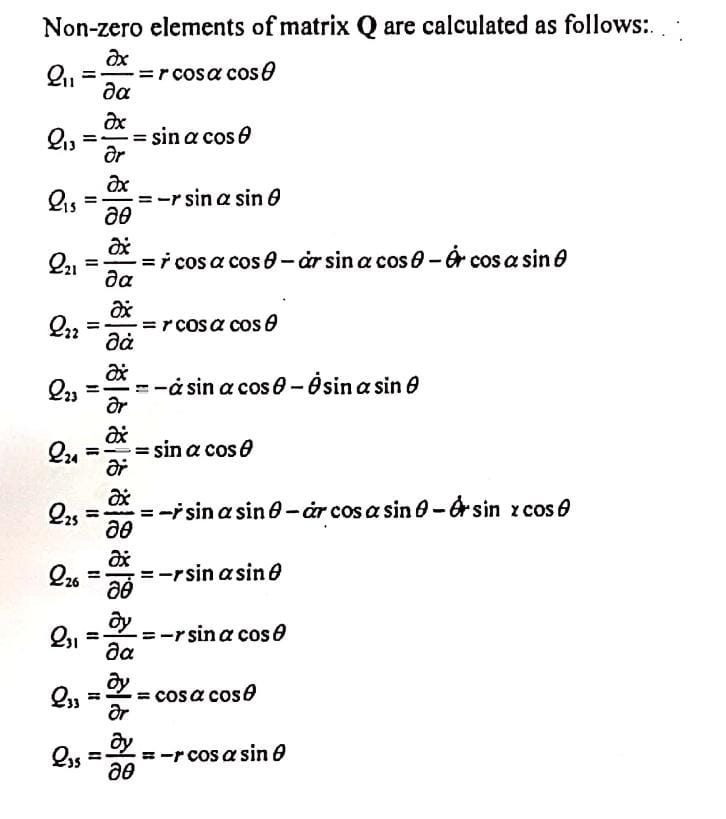
\includegraphics[width=0.5\textwidth,height=0.5\textheight,keepaspectratio]{figures/cartesian-covariance1}
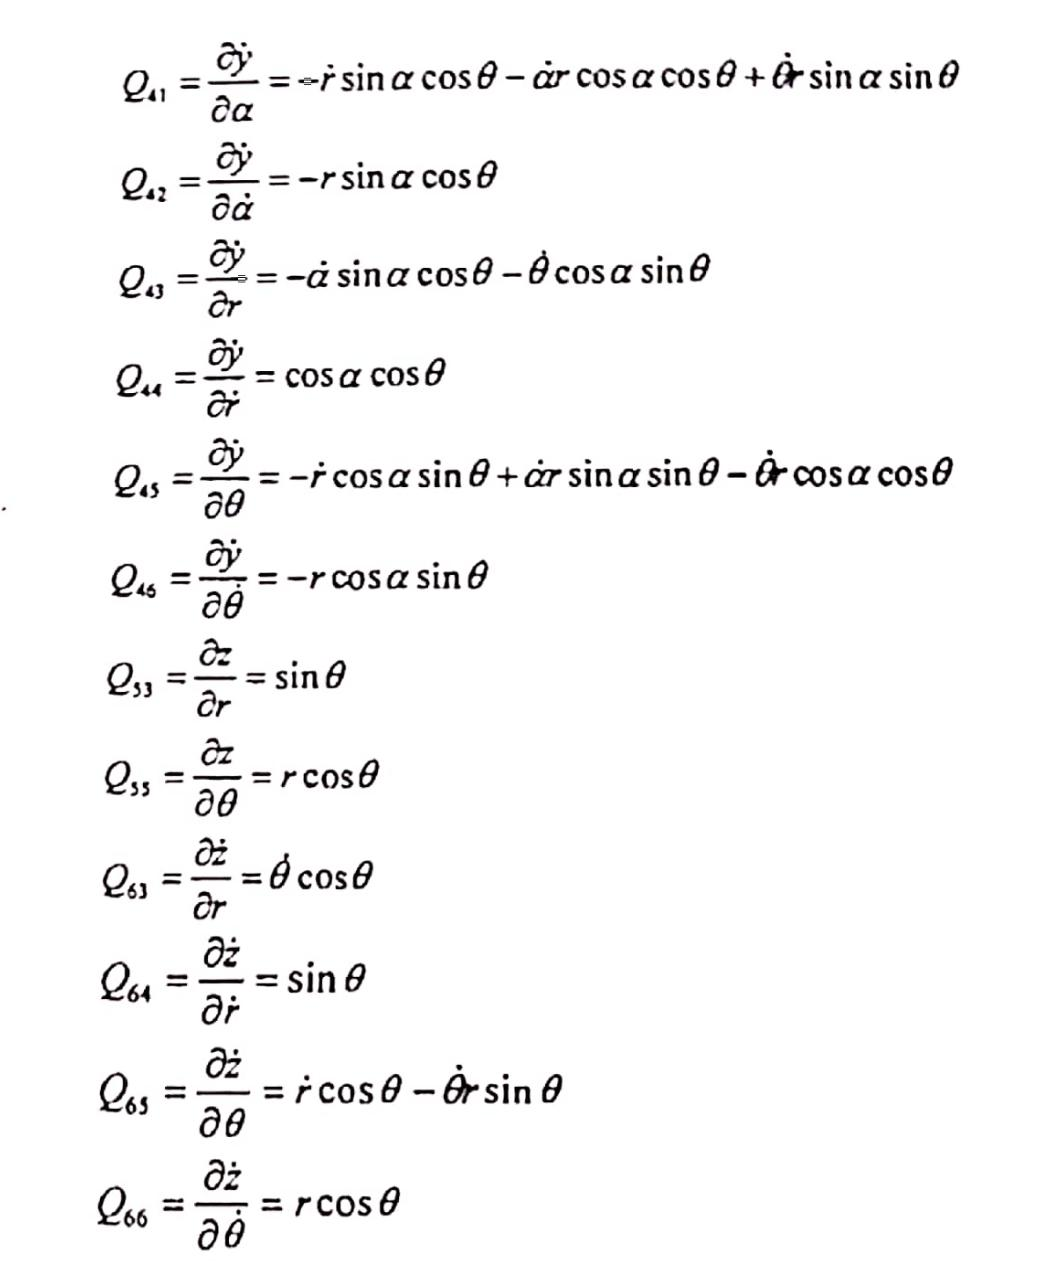
\includegraphics[width=0.5\textwidth,height=0.5\textheight,keepaspectratio]{figures/cartesian-covariance2}
\end{figure}

As described in pages 14-16.


\paragraph{Conversion of covariance from spherical to cartesian:}
Given a diagonal matrix $(x,y,z)$, the jacobian of $(\theta, r, \phi)$ with
respect to $(x,y,z)$ is:


\begin{equation}\label{jacobian:position-cartesian}
\begin{pmatrix}
    \frac{y}{x^2+y^2} & \frac{x}{x^2+y^2} & 0
    \\
    \frac{x}{r} & \frac{y}{r} & \frac{z}{r} \\
    \frac{xz}{r^2\sqrt{x^2+y^2}} & \frac{yz}{r^2\sqrt{x^2+y^2}} &
    \frac{\sqrt{x^2+y^2}}{r^2}
  \end{pmatrix}
\end{equation}


Given a diagonal matrix $(x,\dot{x},y,\dot{y},z,\dot{z})$,the jacobian of
$(x,\dot{x},y,\dot{y},z,\dot{z})$ with respect to $(\theta,\brate, r, \rrate, \phi, \erate)$ is:


\begin{figure}[H]\label{fig:spherical}
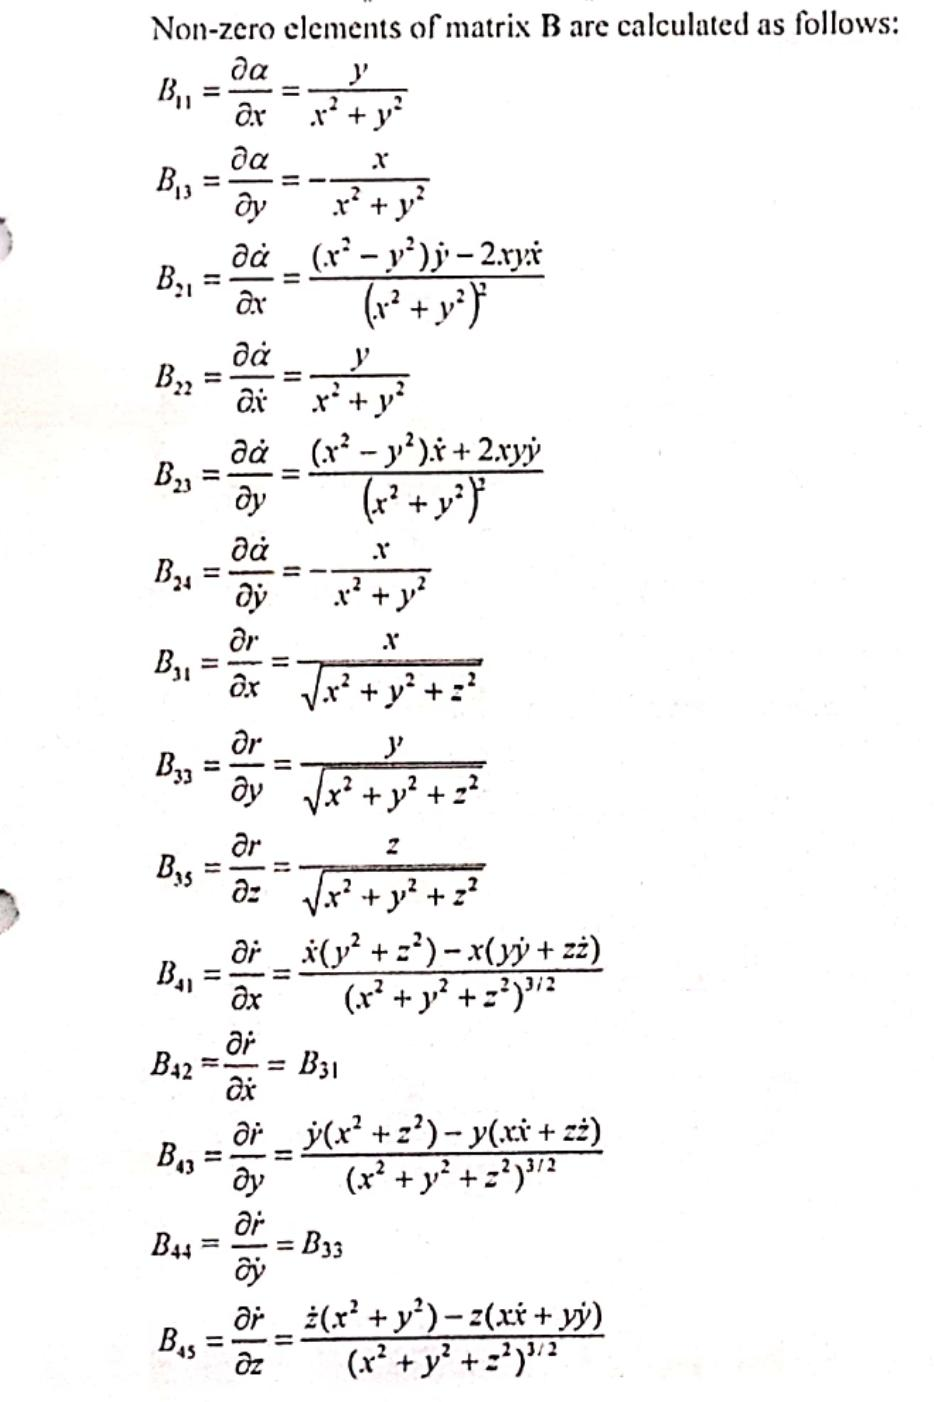
\includegraphics[width=0.5\textwidth,height=0.5\textheight,keepaspectratio]{figures/spherical-covariance1}
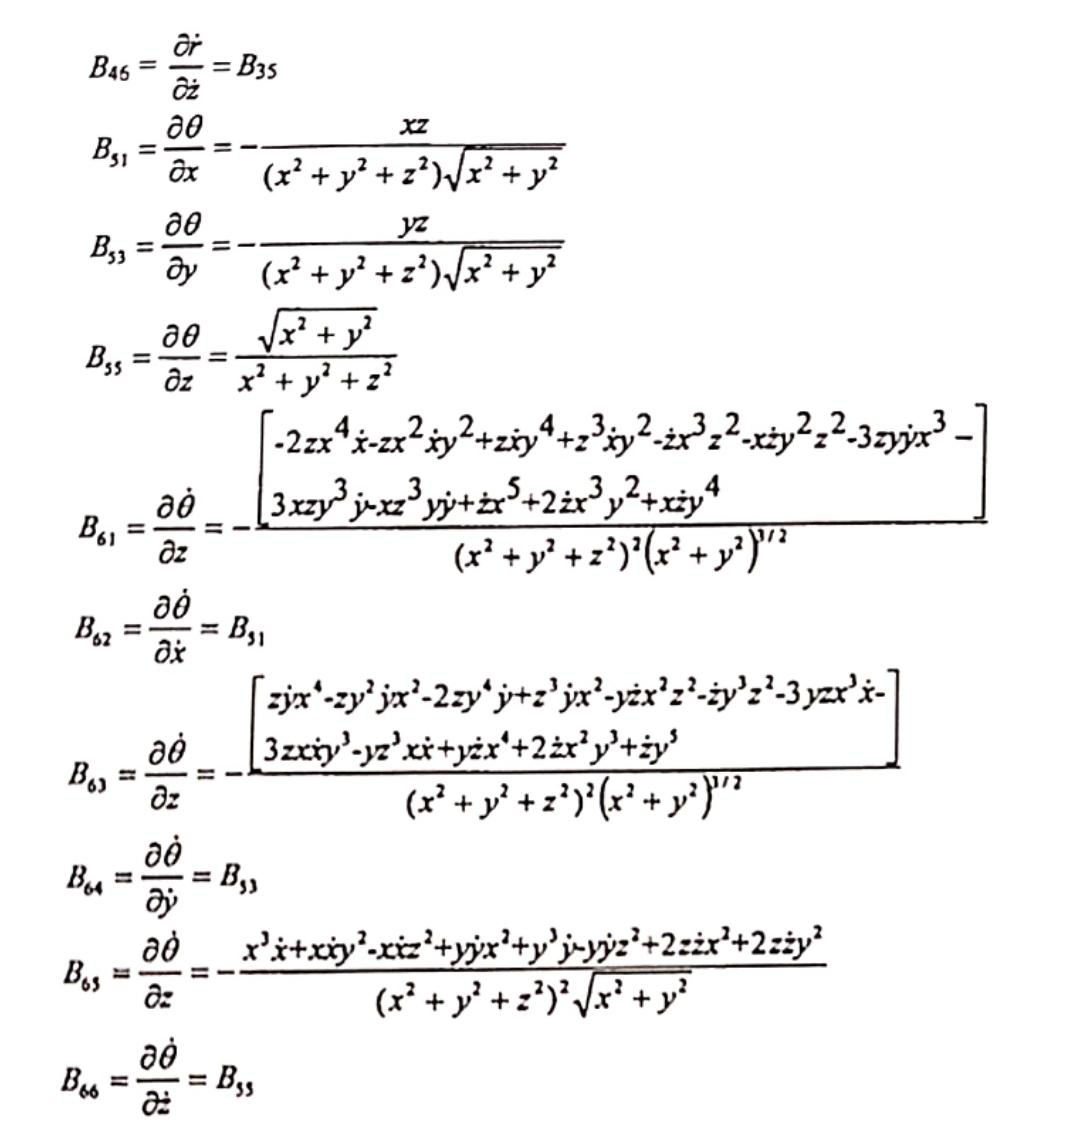
\includegraphics[width=0.5\textwidth,height=0.5\textheight,keepaspectratio]{figures/spherical-covariance2}
\end{figure}

As described in pages 11-13.

%\newpage


\section{Appendix}
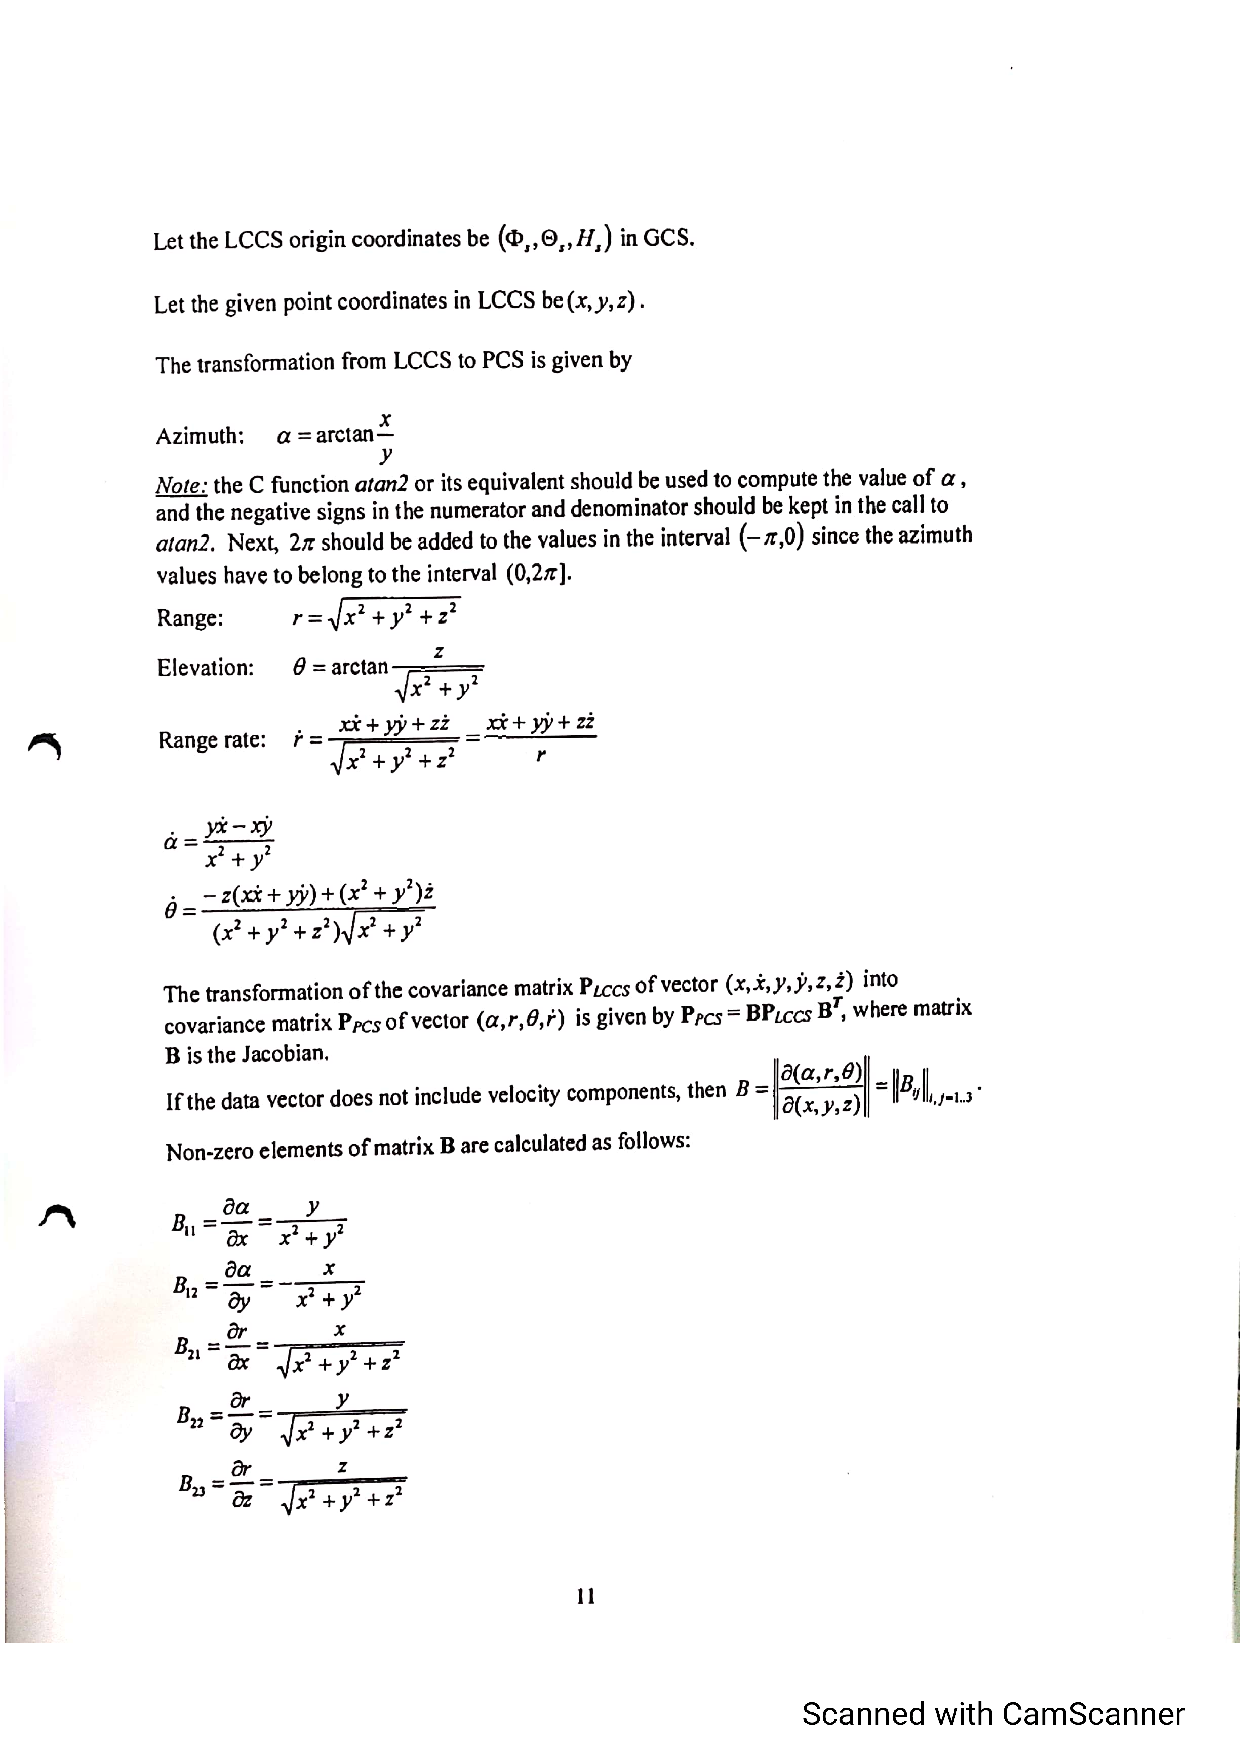
\includepdf[pages=1-6,pagecommand={},width=\textwidth]{tsg/tsg.pdf}

\end{document}
